\documentclass{report_ndr}

\usepackage{lipsum}
% opening
\title{Звіт на тему філософських уявлень Ціцерона про межі добра та зла}

\author{А.В. Тор}

\begin{document}

\maketitle

\tableofcontents

\chapter{Це дуже важливий розділ}

Але щоб ви зрозуміли, звідки виникає це хибне уявлення людей, цуратись насолоди
і вихваляти страждання, я розкрию перед вами всю картину і роз’ясню, що саме
говорив цей чоловік, який відкрив істину, якого я б назвав зодчим щасливого
життя. Дійсно, ніхто не відкидає, не зневажає, не уникає насолод тільки через
те, що це насолоди, але лише через те, що тих, хто не вміє розумно вдаватися
насолоді, осягають великі страждання. Так само як немає нікого, хто полюбивши,
вважав за краще і зажадав би саме страждання тільки за те, що це страждання, а
не тому, що інший раз виникають такі обставини, коли страждання і біль приносять
якесь і чималу насолоду. Якщо скористатися найпростішим прикладом, то хто з нас
став би займатися якими б то не було тяжкими фізичними вправами, якщо б це не
приносило з собою якоїсь користі? І хто міг би по справедливості дорікнути
прагнення до насолоди, яке не несло б з собою ніяких неприємностей, або того,
хто уникав би такого страждання, яке не приносило б з собою ніякої насолоди?

\begin{figure}[h]
\centering
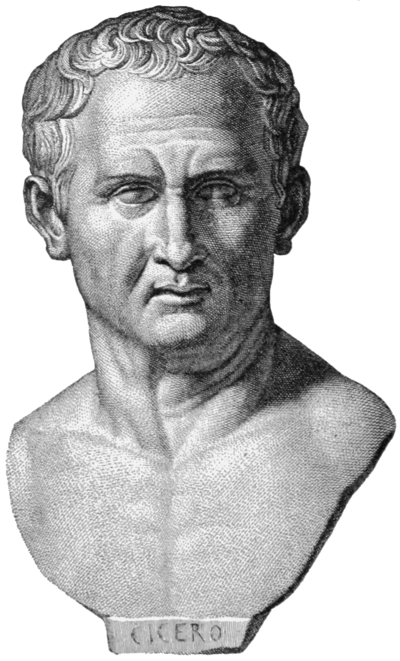
\includegraphics[scale=0.3]{400px-Cicero.PNG}
\caption{Погруддя Ціцерона}
\label{fig:image}
\end{figure}

\chapter{Це не менш важливий розділ. Але, він другий}

Але ми цураємось і вважаємо, що заслуговують справедливого обурення ті, хто,
піддався звабі і розбещеним спокусам, які дають їм насолоду, і без тями від
пристрасті не передбачили, яких страждань і які нещастя на них чекають. Вони
винні так само, як і ті, хто через душевну слабкість, тобто через бажання
уникнути страждань і болю відмовляється від виконання свого обов’язку. Втім, тут
дуже легко і просто провести відмінності, тому що, коли ми вільні і нам надана
повна можливість вибору бажаного, коли ніщо не заважає нам робити те, що нам
більше подобається, будь яку насолоду слід визнати бажаним, а будь-яке
страждання огидним. Але при деяких обставинах – або на вимогу боргу, або в силу
якоїсь необхідності часто доводиться забувати про насолоди і не втікати від
тягарів. Тому мудрець дотримується в цьому випадку наступного принципу вибору –
або, відмовляючись від задоволення, він отримує якісь інші і навіть великі
насолоди, або, зазнаючи страждання, він позбавляється від більш жорстоких.

\begin{table}[h!]
    \caption{Таблиця чогось цікавого}
    \centering
    \begin{tabular}{| l | l | l |}
    \hline
    Назва & Дата & Розмір у папугах \\ \hline
    Бегемот & 11.01.2021 & 83,6 \\ \hline
    Носоріг & 11.01.2021 & 79,4 \\ \hline
    Удав & 1 11.01.2021 & 508,3 \\
    \hline
    \end{tabular}
\end{table}

\section*{А це ще якийсь англійський текст без нумерації}

\lipsum[1-2]

\begin{appendices}

\append{Якийсь важливий додаток}

\lipsum[3-8]

\section{Заголовок пунктy додатку}

\lipsum[9]

\append{Інший важливий додаток}

\lipsum[10-12]

\end{appendices}

\end{document}
